% Use only LaTeX2e, calling the article.cls class and 12-point type.

\documentclass[12pt]{article}

\usepackage{times}

% Packages I manually added
\usepackage{graphicx}
\usepackage{placeins}
\usepackage{float}
\usepackage{amsmath}
\usepackage{hyperref}

\topmargin 0.0cm
\oddsidemargin 0.2cm
\textwidth 16cm
\textheight 21cm
\footskip 1.0cm


% The preamble here sets up a lot of new/revised commands and
% environments.  It's annoying, but please do *not* try to strip these
% out into a separate .sty file (which could lead to the loss of some
% information when we convert the file to other formats).  Instead, keep
% them in the preamble of your main LaTeX source file.


% The following parameters seem to provide a reasonable page setup.

% Include your paper's title here

\title{Supplementary Materials for: ``Well-Designed Environmental Markets Enable Large-Scale Marine Conservation''}


% Place the author information here.  Please hand-code the contact
% information and notecalls; do *not* use \footnote commands.  Let the
% author contact information appear immediately below the author names
% as shown.  We would also prefer that you don't change the type-size
% settings shown here.

\author{Juan Carlos Villase\~{n}or-Derbez,$^{1\ast}$ John Lynham,$^{2}$ Christopher Costello$^{1}$\\
\\
\normalsize{$^{1}$Bren School of Environmental Science \& Management,}\\
\normalsize{University of California at Santa Barbara, Santa Barbara, CA}\\
\normalsize{$^{2}$Department of Economics, University of Hawaii at Manoa, Honolulu, HI}\\
\\
\normalsize{$^\ast$To whom correspondence should be addressed; E-mail: juancarlos@ucsb.edu.}
}

% Include the date command, but leave its argument blank.

\date{}



%%%%%%%%%%%%%%%%% END OF PREAMBLE %%%%%%%%%%%%%%%%

\begin{document}

% Double-space the manuscript.

\baselineskip24pt

% Make the title.

\maketitle

\newcommand{\beginsupplement}{\setcounter{table}{0}  \renewcommand{\thetable}{S\arabic{table}} \setcounter{figure}{0} \renewcommand{\thefigure}{S\arabic{figure}}}

\setcounter{table}{0}  \renewcommand{\thetable}{S\arabic{table}} \setcounter{figure}{0} \renewcommand{\thefigure}{S\arabic{figure}}

\section{Supplementary Materials}

\subsection{Model parameterization}

We calibrate our model to loosely match the fishery dynamics observed for the VDS operated by the PNA. The table below contains the values used to parameterize the model.

\begin{table}[H]
\centering
\resizebox{\linewidth}{!}{
\begin{tabular}{l|r|l}
\hline
Parameter & Value & Source\\
\hline
MSY & 1.875600e+06 & 50th percentile from MSY in Table 8 of WCPFC Stock Assessment\\
\hline
$B_{msy}$ & 1.628000e+06 & 50th percentile from MSY in Table 8 of WCPFC Stock Assessment\\
\hline
K & 6.876526e+06 & 50th percentile from MSY in Table 8 of WCPFC Stock Assessment\\
\hline
$B_c/B_{msy}$ & 0.51 & 50th percentile from MSY in Table 8 of WCPFC Stock Assessment\\
\hline
$C_{now}$ & 1.679444e+06 & Catches from WCPFC Stock Assessment\\
\hline
$B_{now}$ & 3.507028e+06 & Current Biomass (2012 - 2015 average)\\
\hline
$r$ & 0.57 & From FishBase: Prior r = 0.57, 95 CL = 0.41 - 0.78\\
\hline
$\beta$ & 1.3 & Standard\\
\hline
p & 1100 & Mean between Thailand and Japan values (Value of WCPFC-CA Tuna Fisheries 2017 Report)\\
\hline
q & 3.420000e-05 & Estimated so that efforts match catches given biomass and vessel-day prices\\
\hline
c & 1800 & Estimated to match cost and revenue structures\\
\hline
f & 0.1 & Biomass is equally distributed between countries\\
\hline
\end{tabular}}
\end{table}


\subsection{Empirical Analysis}

\subsubsection{Effort redistribution}

We can compare the footprint of displaced and non-displaced vessels before and after the implementation of PIPA to better understand the effort redistribution. Non-displaced vessels serve as a control group that was not subject to a spatial closure but might have redistributed in response to changing environmental conditions, such as ENSO. The spatial redistribution patterns of displaced vessels relative to non-displaced vessels suggest that some relocated to other waters in Kiribati (\emph{i.e.} Gilbert islands and Line islands), but also the Marshall Islands, Tuvalu, Nauru, and the high seas (Fig \ref{fig:fishing_raster_diff}).

\subsubsection{Data and code availability}

Raw data and code used in this work are available on \href{https://github.com/jcvdav/MPA_displacement}{github}.

\clearpage

\FloatBarrier

\section{Supplementary tables and figures}

\begin{figure}[htbp]
\centering
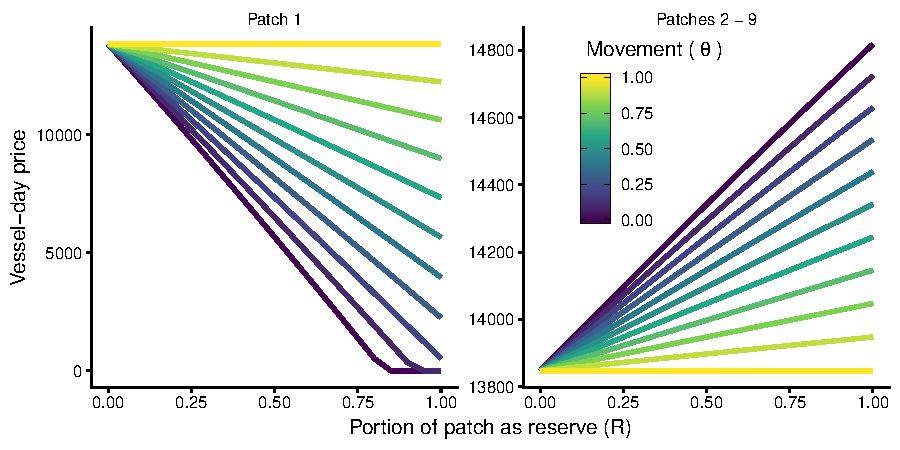
\includegraphics{img/vessel_day_price_no_trading_plot.pdf}
\caption{\label{fig:vessel_day_price_no_trading_plot}Vessel-day prices (vertical axis) for a combination of reserve sizes ($R$ in the horizontal-axis) and different within-country movement ($\theta$) for the country with spatial closure and other countries (left - right, respectively) when there is no trading.}
\end{figure}

\begin{figure}[htbp]
\centering
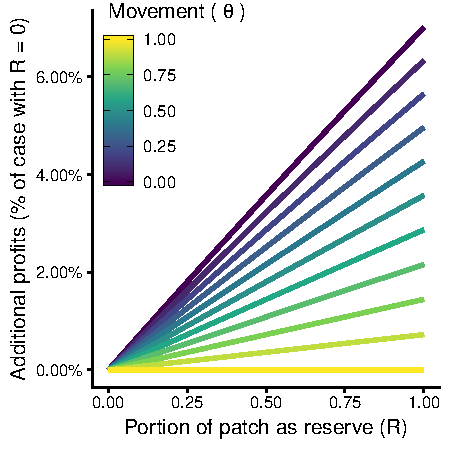
\includegraphics{img/profits_PNA_notKIR_no_trading_plot.pdf}
\caption{\label{fig:profits_PNA_notKIR_no_trading_plot}Relative change in revenue for countries 2 - 9 (vertical axis) for a combination of reserve sizes ($R$ in the horizontal-axis) and different within-country movement ($\theta$) when there is no trading.}
\end{figure}

\begin{figure}
\centering
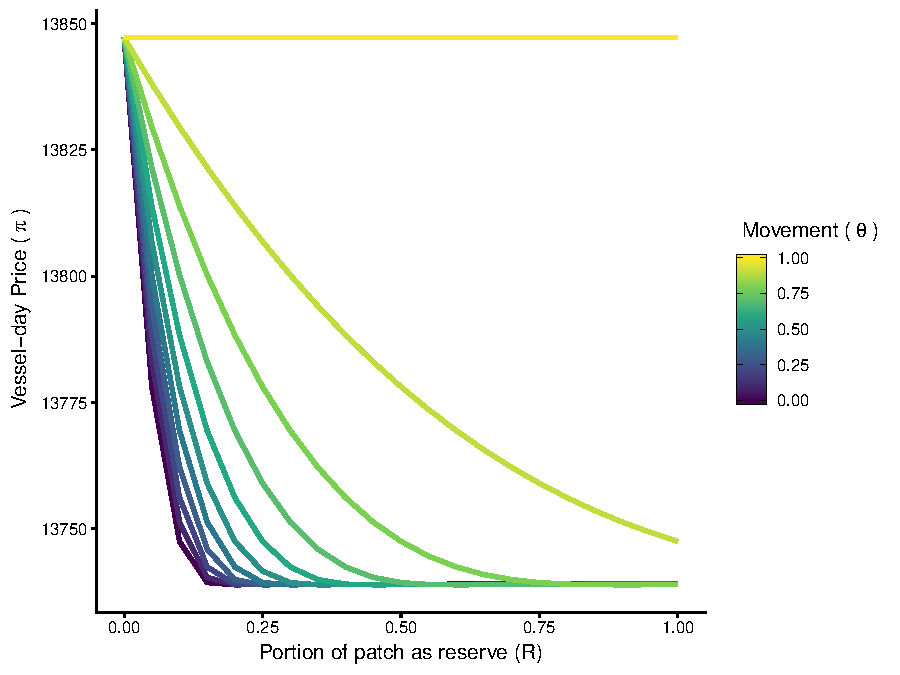
\includegraphics{img/vessel_day_price_with_trading_plot.pdf}
\caption{\label{fig:vessel_day_price_with_trading_plot}PNA-wide vessel-day prices (vertical axis) with trading, for a combination of reserve sizes ($R$ in the horizontal-axis) and different within-country movement ($\theta$).}
\end{figure}

\begin{figure}
	\centering
	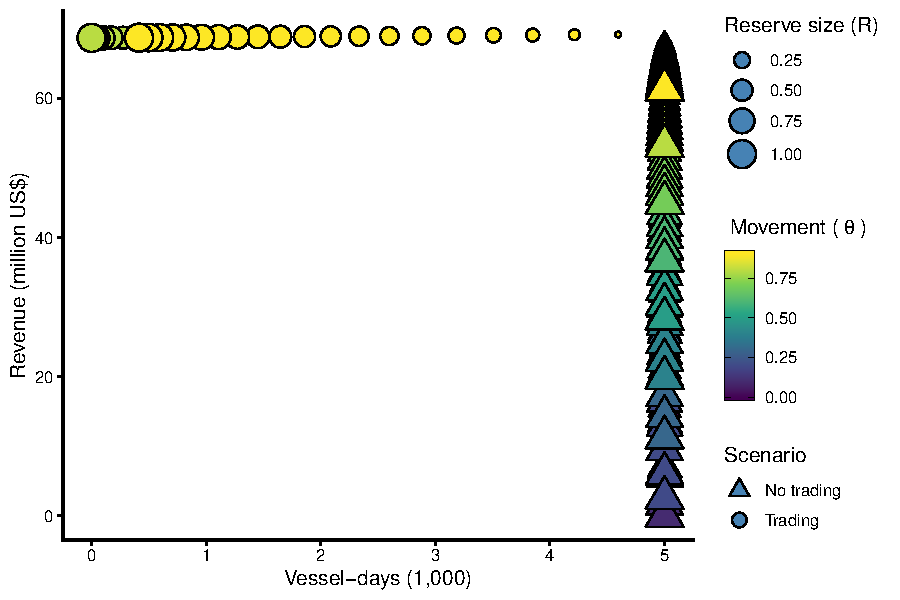
\includegraphics{img/effort_and_revenues.pdf}
	\caption{\label{fig:effort_and_revenues}Effort and revenue in Patch 1 for a combination of reserve sizes ($R$), different within-country movement ($\theta$), and with and without trading. With trading, the relative drop in effort is always larger than the relative drop in revenue as $R$ increases. The exact opposite relationship holds without trading: effort remains fixed as revenue declines with increasing $R$.}
\end{figure}

\begin{figure}
\centering
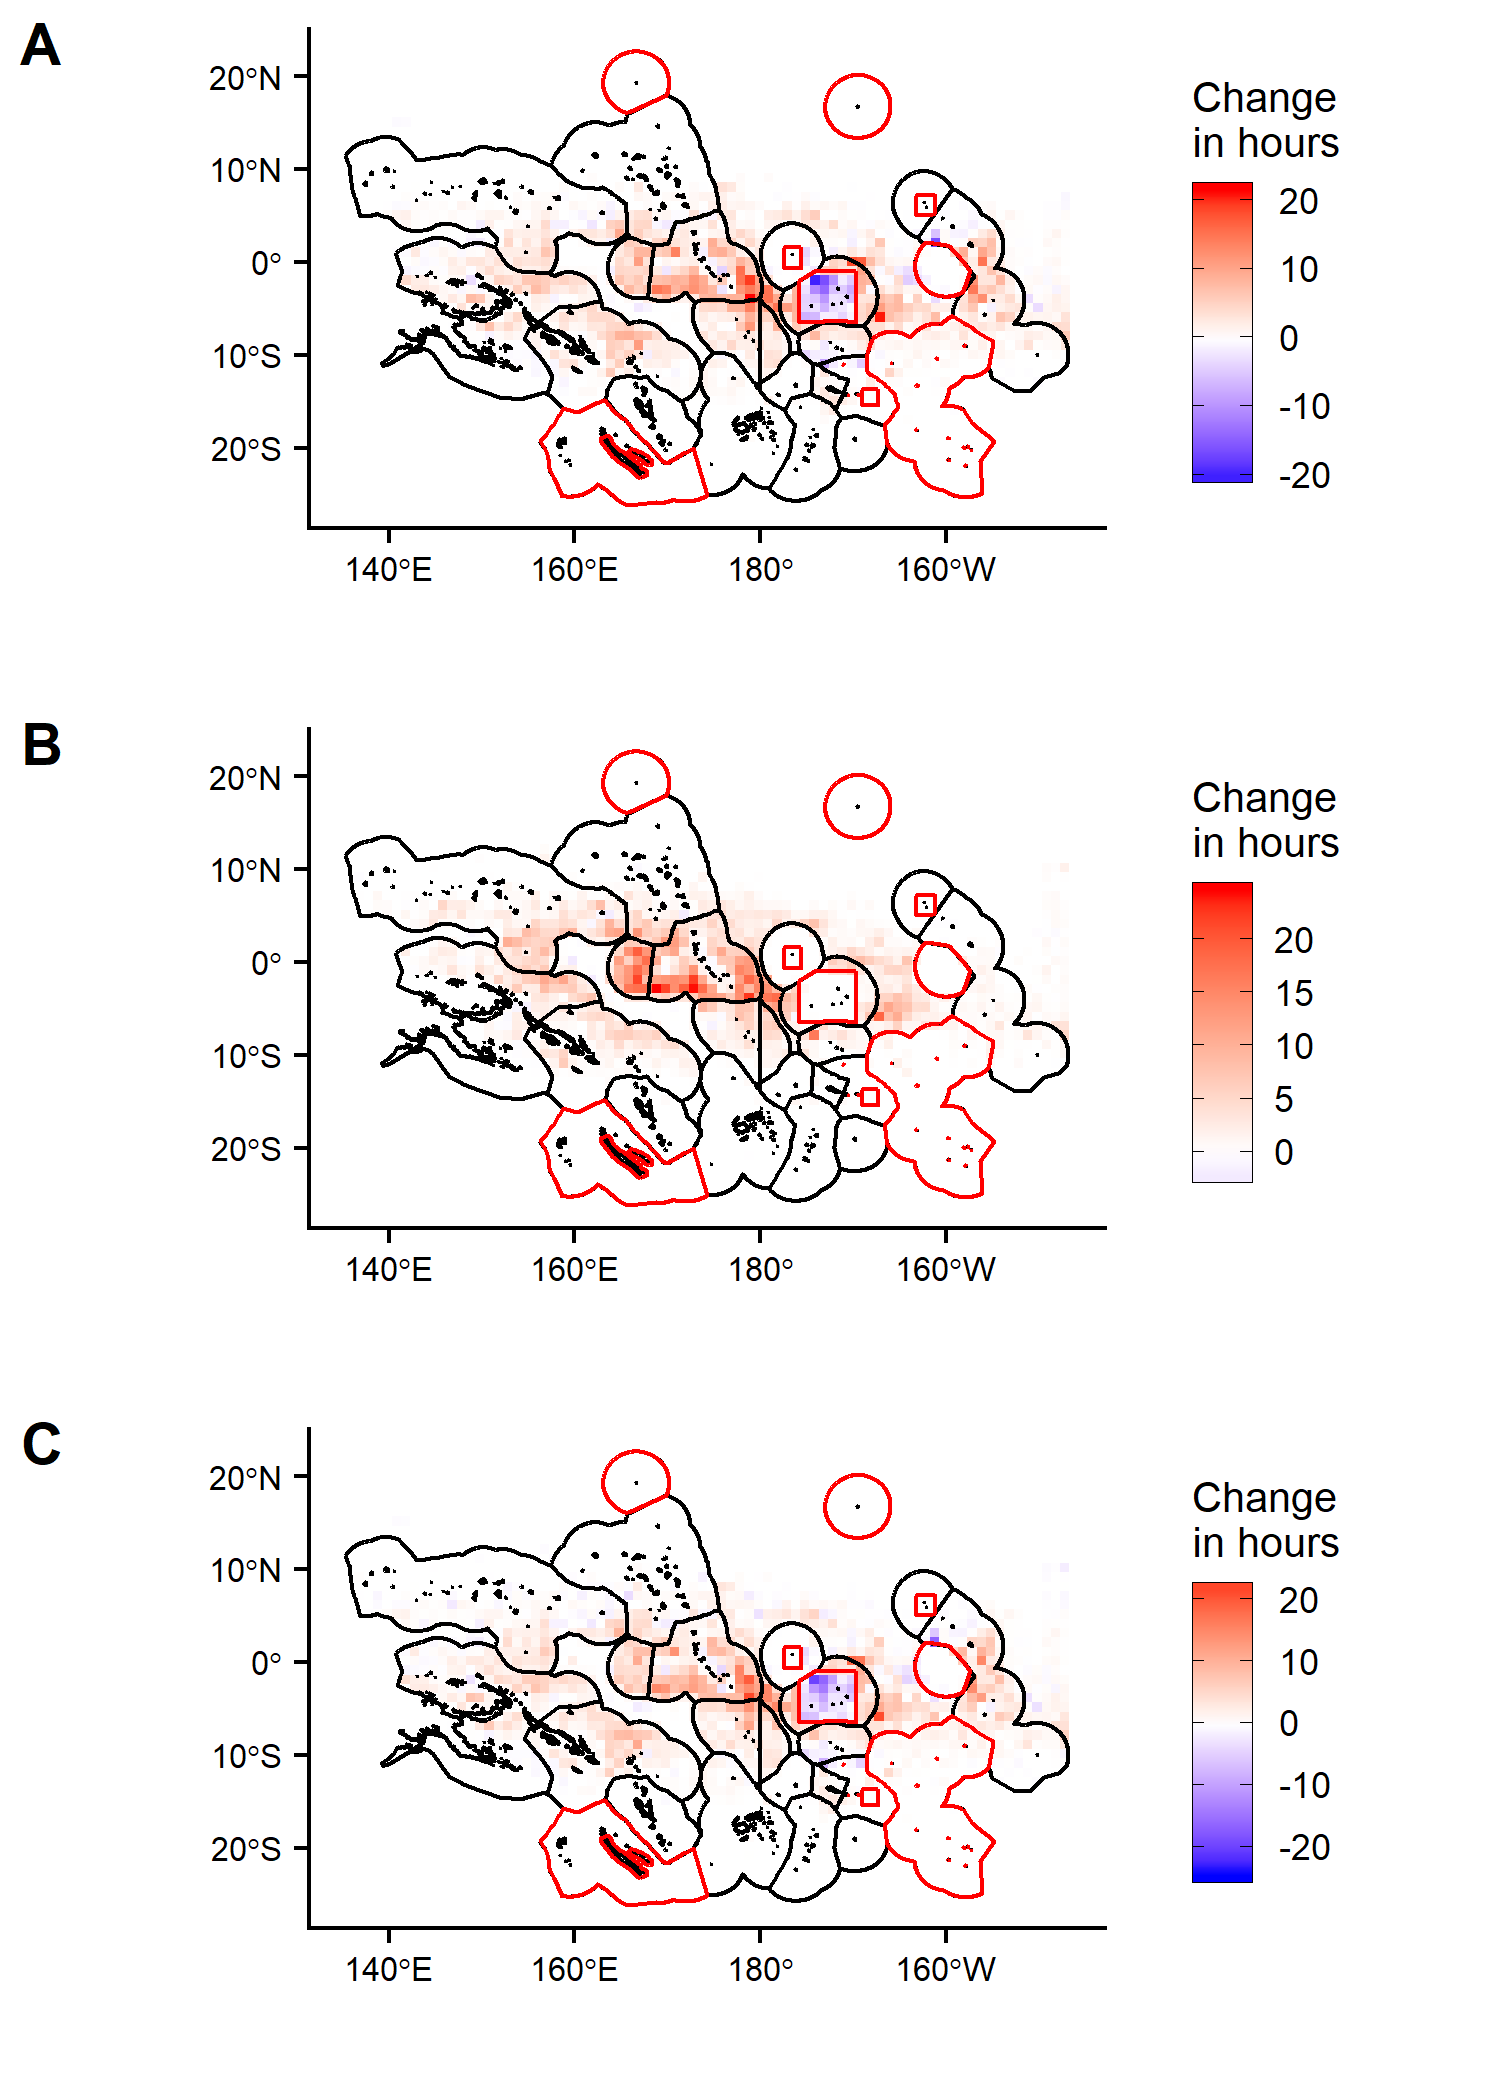
\includegraphics{img/fishing_raster_diff.png}
\caption{\label{fig:fishing_raster_diff}Change in spatial footprint of analyzed vessels. Black lines show Exclusive Economic Zone (EEZ), red lines show Marine Protected Areas. Panels A and B show the change through time (after - before) for displaced (A) and non-displaced vessels (B). Panel C shows the difference between A and B (displaced - non-displaced), highlighting areas where displaced vessels redistributed to, relative to non-displaced vessels. Note that displaced vessels allocate more hours to the Gilbert Islands and Line islands EEZs, but also Tuvalu and the high seas surrounding PIPA and Kiribati's EEZ.}
\end{figure}

\begin{figure}
\centering
	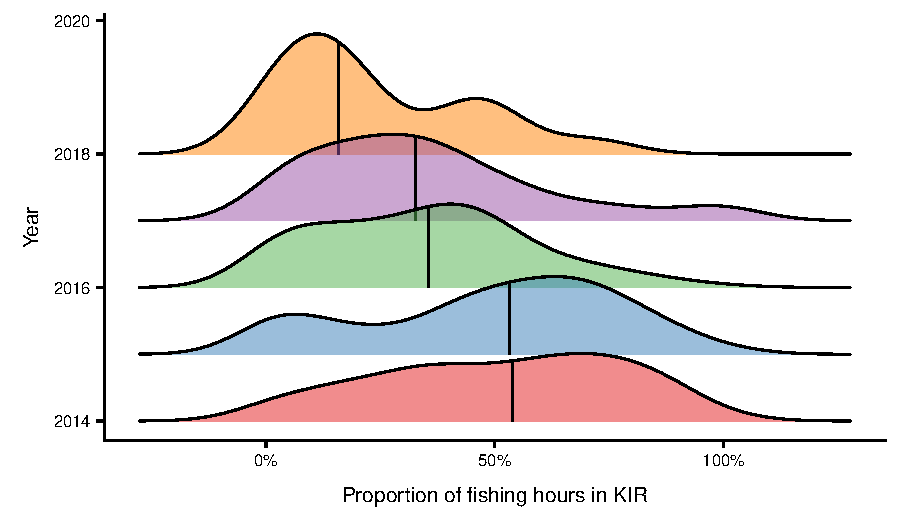
\includegraphics{img/hist_kir_fishing.pdf}
	\caption{\label{fig:hist_kir_fishing}Ridgeplot for the density of the \% of total fishing hours that took place within Kiribati EEZ waters by year for displaced vessels where the unit of observation is an individual vessel. The vertical lines represent the median of each year.}	
\end{figure}

\begin{figure}
\centering
	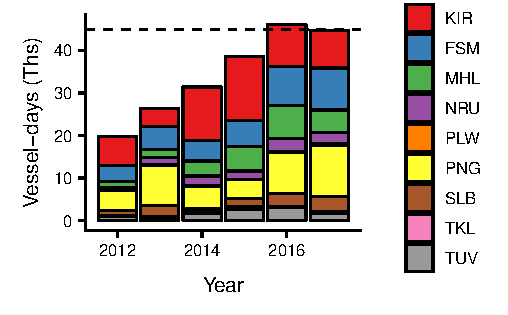
\includegraphics{img/all_PS_VDS_cty_year.pdf}
	\caption{\label{fig:all_PS_VDS_cty_year}Annual vessel-days for all PNA countries, by country.}
\end{figure}

\begin{figure}
\centering
	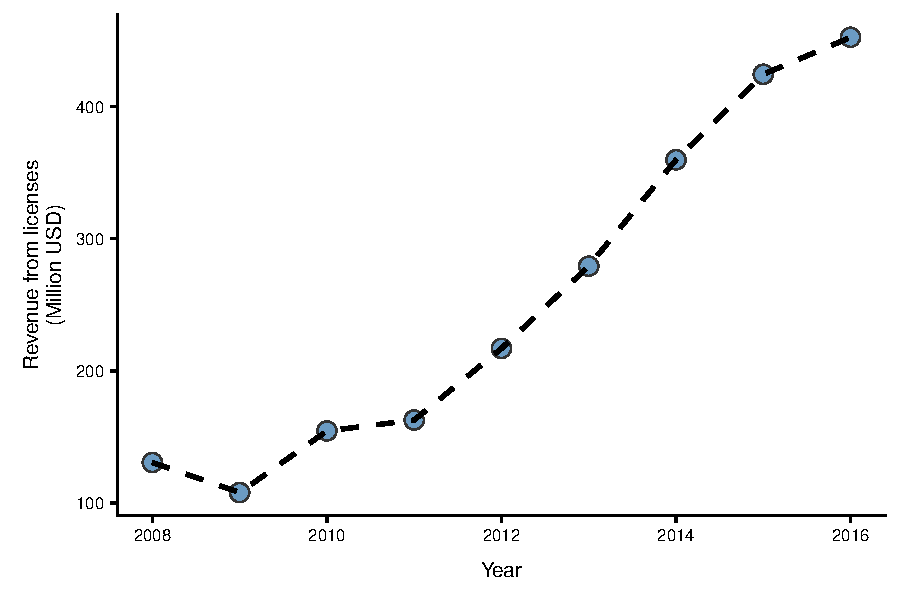
\includegraphics{img/total_PNA_revenues.pdf}
	\caption{\label{fig:total_PNA_revenues}Total revenues for all PNA countries combined.}
\end{figure}

\begin{figure}
\centering
	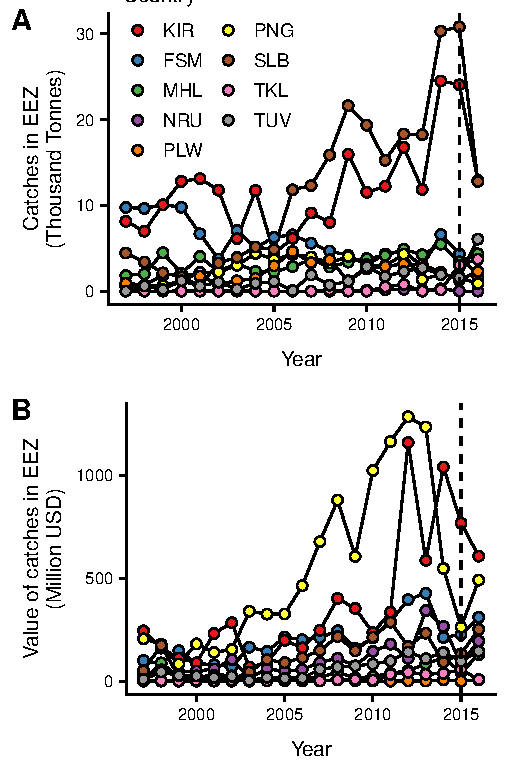
\includegraphics{img/catches.pdf}
	\caption{\label{fig:catches}Financial indicators for PNA countries. A) Total annual purse seine catch by EEZ and, B) Total annual value of purse seine catch by EEZ. Vertical dashed line in both plots denotes implementation of PIPA.}
\end{figure}

\begin{figure}
\centering
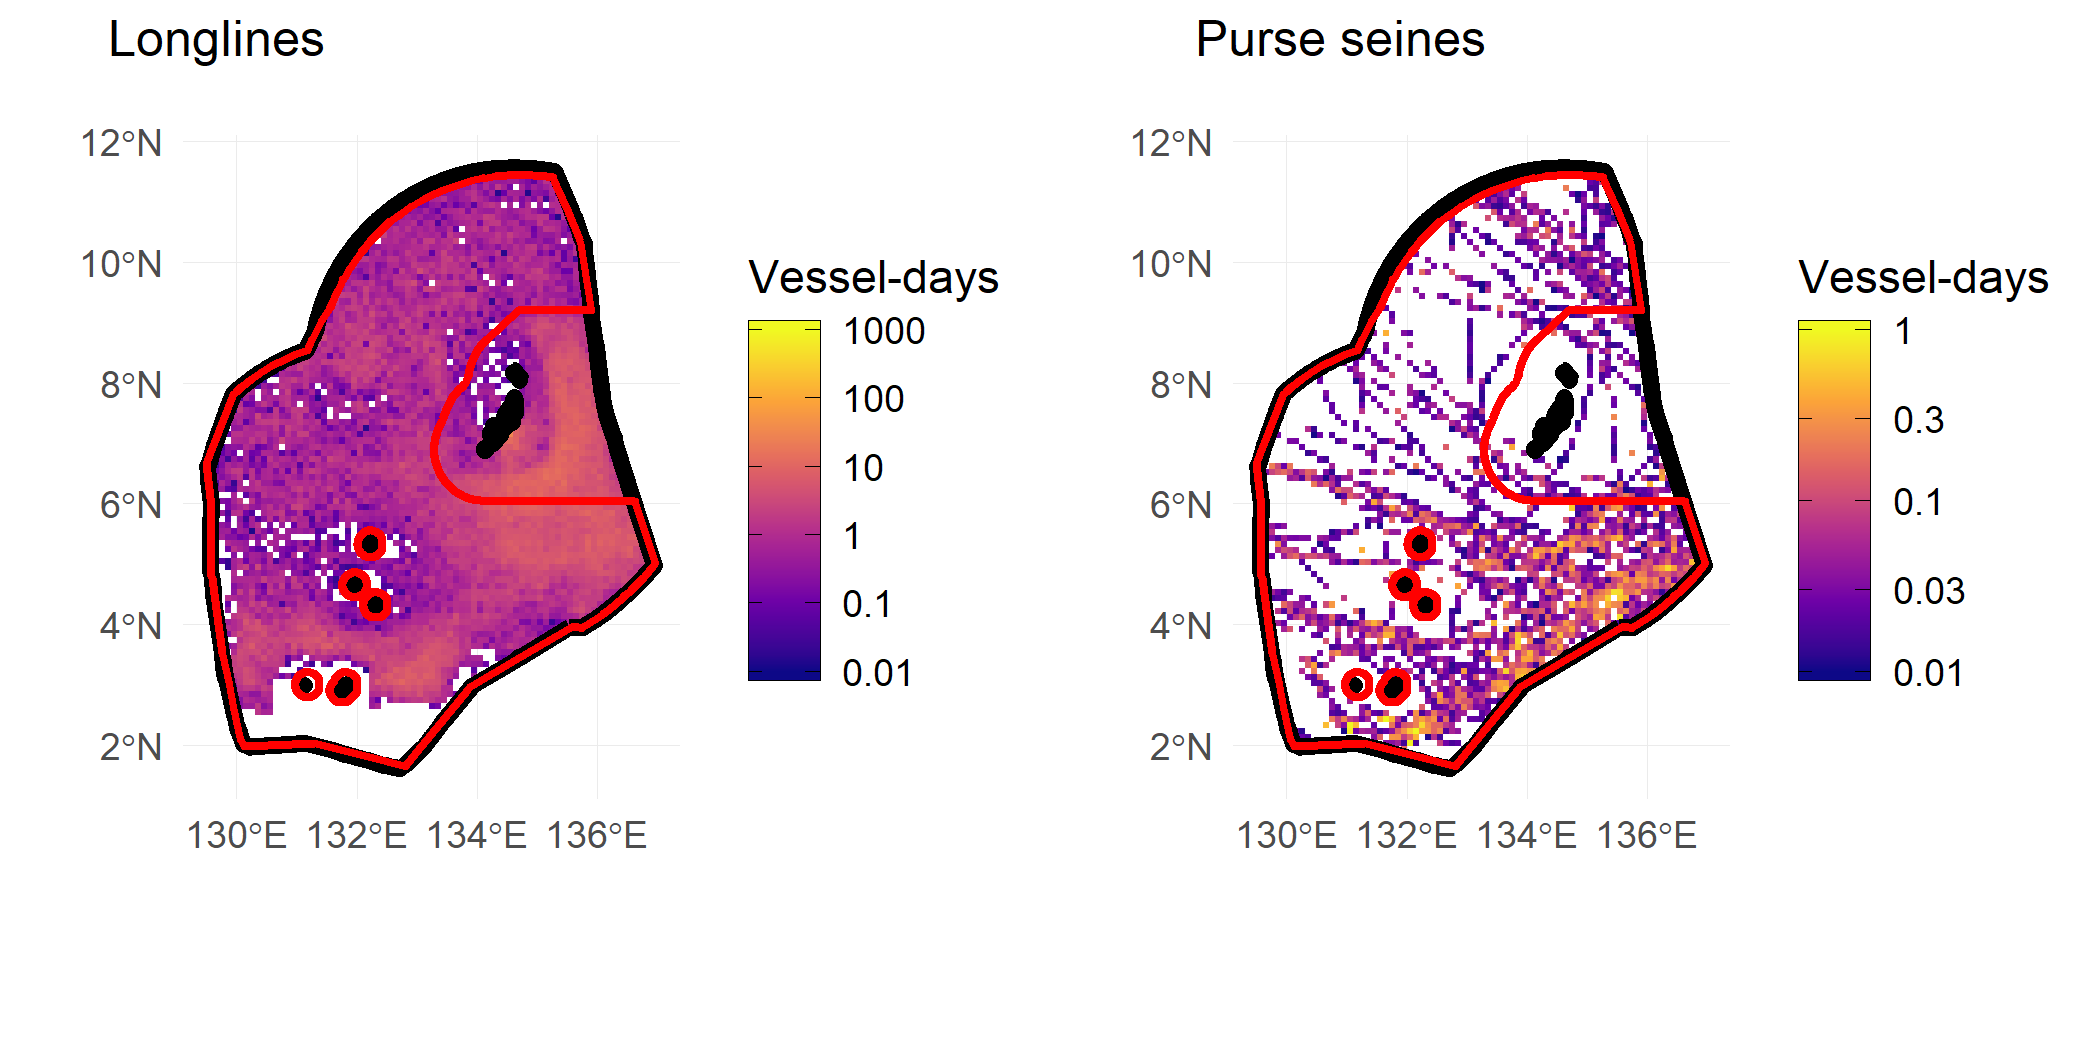
\includegraphics{img/plw_2018.png}
\caption{\label{fig:plw_2018}Longline and purse seine fishing effort in Palau during 2018 at a 0.5 degree resolution. The red polygon shows the proposed Palau National Marine Sanctuary, containing 56\% and 91\% of longline and purse seine fishing effort, respectively. Note that the colorbars are presented in $log_{10}$ transformed scale for better visualization.}
\end{figure}

\begin{figure}
\centering
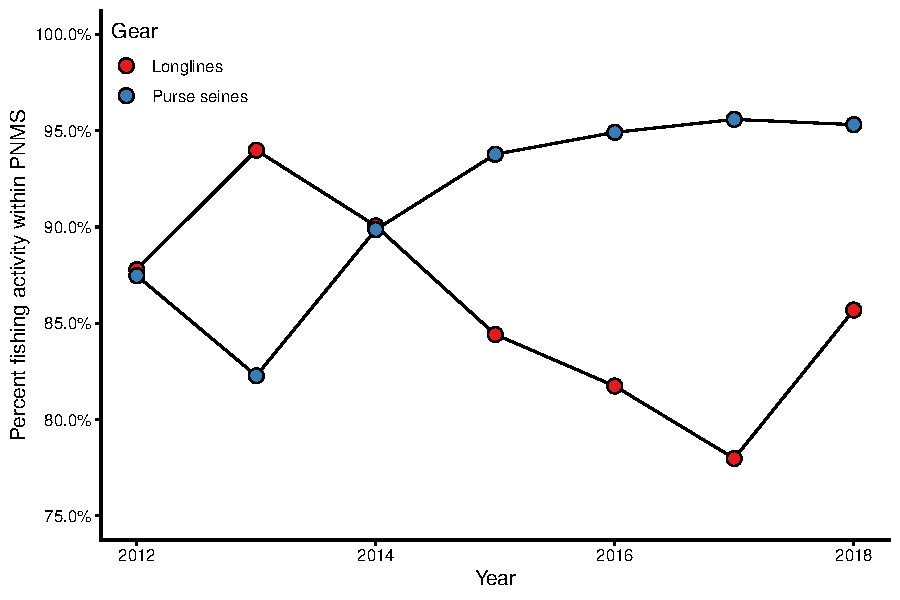
\includegraphics{img/plw_ts_plot.pdf}
\caption{\label{fig:plw_ts_plot}Time series of the annual proportion of longline and purse seine effort within the proposed PNMS boundaries.}
\end{figure}

\clearpage

\end{document}
